% Options for packages loaded elsewhere
\PassOptionsToPackage{unicode}{hyperref}
\PassOptionsToPackage{hyphens}{url}
%
\documentclass[
]{article}
\usepackage{amsmath,amssymb}
\usepackage{iftex}
\ifPDFTeX
  \usepackage[T1]{fontenc}
  \usepackage[utf8]{inputenc}
  \usepackage{textcomp} % provide euro and other symbols
\else % if luatex or xetex
  \usepackage{unicode-math} % this also loads fontspec
  \defaultfontfeatures{Scale=MatchLowercase}
  \defaultfontfeatures[\rmfamily]{Ligatures=TeX,Scale=1}
\fi
\usepackage{lmodern}
\ifPDFTeX\else
  % xetex/luatex font selection
\fi
% Use upquote if available, for straight quotes in verbatim environments
\IfFileExists{upquote.sty}{\usepackage{upquote}}{}
\IfFileExists{microtype.sty}{% use microtype if available
  \usepackage[]{microtype}
  \UseMicrotypeSet[protrusion]{basicmath} % disable protrusion for tt fonts
}{}
\makeatletter
\@ifundefined{KOMAClassName}{% if non-KOMA class
  \IfFileExists{parskip.sty}{%
    \usepackage{parskip}
  }{% else
    \setlength{\parindent}{0pt}
    \setlength{\parskip}{6pt plus 2pt minus 1pt}}
}{% if KOMA class
  \KOMAoptions{parskip=half}}
\makeatother
\usepackage{xcolor}
\usepackage[margin=1in]{geometry}
\usepackage{color}
\usepackage{fancyvrb}
\newcommand{\VerbBar}{|}
\newcommand{\VERB}{\Verb[commandchars=\\\{\}]}
\DefineVerbatimEnvironment{Highlighting}{Verbatim}{commandchars=\\\{\}}
% Add ',fontsize=\small' for more characters per line
\usepackage{framed}
\definecolor{shadecolor}{RGB}{248,248,248}
\newenvironment{Shaded}{\begin{snugshade}}{\end{snugshade}}
\newcommand{\AlertTok}[1]{\textcolor[rgb]{0.94,0.16,0.16}{#1}}
\newcommand{\AnnotationTok}[1]{\textcolor[rgb]{0.56,0.35,0.01}{\textbf{\textit{#1}}}}
\newcommand{\AttributeTok}[1]{\textcolor[rgb]{0.13,0.29,0.53}{#1}}
\newcommand{\BaseNTok}[1]{\textcolor[rgb]{0.00,0.00,0.81}{#1}}
\newcommand{\BuiltInTok}[1]{#1}
\newcommand{\CharTok}[1]{\textcolor[rgb]{0.31,0.60,0.02}{#1}}
\newcommand{\CommentTok}[1]{\textcolor[rgb]{0.56,0.35,0.01}{\textit{#1}}}
\newcommand{\CommentVarTok}[1]{\textcolor[rgb]{0.56,0.35,0.01}{\textbf{\textit{#1}}}}
\newcommand{\ConstantTok}[1]{\textcolor[rgb]{0.56,0.35,0.01}{#1}}
\newcommand{\ControlFlowTok}[1]{\textcolor[rgb]{0.13,0.29,0.53}{\textbf{#1}}}
\newcommand{\DataTypeTok}[1]{\textcolor[rgb]{0.13,0.29,0.53}{#1}}
\newcommand{\DecValTok}[1]{\textcolor[rgb]{0.00,0.00,0.81}{#1}}
\newcommand{\DocumentationTok}[1]{\textcolor[rgb]{0.56,0.35,0.01}{\textbf{\textit{#1}}}}
\newcommand{\ErrorTok}[1]{\textcolor[rgb]{0.64,0.00,0.00}{\textbf{#1}}}
\newcommand{\ExtensionTok}[1]{#1}
\newcommand{\FloatTok}[1]{\textcolor[rgb]{0.00,0.00,0.81}{#1}}
\newcommand{\FunctionTok}[1]{\textcolor[rgb]{0.13,0.29,0.53}{\textbf{#1}}}
\newcommand{\ImportTok}[1]{#1}
\newcommand{\InformationTok}[1]{\textcolor[rgb]{0.56,0.35,0.01}{\textbf{\textit{#1}}}}
\newcommand{\KeywordTok}[1]{\textcolor[rgb]{0.13,0.29,0.53}{\textbf{#1}}}
\newcommand{\NormalTok}[1]{#1}
\newcommand{\OperatorTok}[1]{\textcolor[rgb]{0.81,0.36,0.00}{\textbf{#1}}}
\newcommand{\OtherTok}[1]{\textcolor[rgb]{0.56,0.35,0.01}{#1}}
\newcommand{\PreprocessorTok}[1]{\textcolor[rgb]{0.56,0.35,0.01}{\textit{#1}}}
\newcommand{\RegionMarkerTok}[1]{#1}
\newcommand{\SpecialCharTok}[1]{\textcolor[rgb]{0.81,0.36,0.00}{\textbf{#1}}}
\newcommand{\SpecialStringTok}[1]{\textcolor[rgb]{0.31,0.60,0.02}{#1}}
\newcommand{\StringTok}[1]{\textcolor[rgb]{0.31,0.60,0.02}{#1}}
\newcommand{\VariableTok}[1]{\textcolor[rgb]{0.00,0.00,0.00}{#1}}
\newcommand{\VerbatimStringTok}[1]{\textcolor[rgb]{0.31,0.60,0.02}{#1}}
\newcommand{\WarningTok}[1]{\textcolor[rgb]{0.56,0.35,0.01}{\textbf{\textit{#1}}}}
\usepackage{graphicx}
\makeatletter
\def\maxwidth{\ifdim\Gin@nat@width>\linewidth\linewidth\else\Gin@nat@width\fi}
\def\maxheight{\ifdim\Gin@nat@height>\textheight\textheight\else\Gin@nat@height\fi}
\makeatother
% Scale images if necessary, so that they will not overflow the page
% margins by default, and it is still possible to overwrite the defaults
% using explicit options in \includegraphics[width, height, ...]{}
\setkeys{Gin}{width=\maxwidth,height=\maxheight,keepaspectratio}
% Set default figure placement to htbp
\makeatletter
\def\fps@figure{htbp}
\makeatother
\setlength{\emergencystretch}{3em} % prevent overfull lines
\providecommand{\tightlist}{%
  \setlength{\itemsep}{0pt}\setlength{\parskip}{0pt}}
\setcounter{secnumdepth}{-\maxdimen} % remove section numbering
\ifLuaTeX
  \usepackage{selnolig}  % disable illegal ligatures
\fi
\usepackage{bookmark}
\IfFileExists{xurl.sty}{\usepackage{xurl}}{} % add URL line breaks if available
\urlstyle{same}
\hypersetup{
  pdftitle={EVEN MORE conditional relationships},
  pdfauthor={Prof.~Weldzius},
  hidelinks,
  pdfcreator={LaTeX via pandoc}}

\title{EVEN MORE conditional relationships}
\usepackage{etoolbox}
\makeatletter
\providecommand{\subtitle}[1]{% add subtitle to \maketitle
  \apptocmd{\@title}{\par {\large #1 \par}}{}{}
}
\makeatother
\subtitle{Homework}
\author{Prof.~Weldzius}
\date{Due Date: 2024-09-25}

\begin{document}
\maketitle

\section{Recap}\label{recap}

Recall that we have tested Trump's theory that the MSM was biased
against him. We found that polls that underpredicted Trump \textbf{also}
underpredicted Biden. This is not what we would expect if the polls
favored one candidate over another.

\section{Loading the data}\label{loading-the-data}

\begin{Shaded}
\begin{Highlighting}[]
\FunctionTok{require}\NormalTok{(tidyverse)}
\FunctionTok{require}\NormalTok{(scales)}
\NormalTok{Pres2020.PV }\OtherTok{\textless{}{-}} \FunctionTok{read\_rds}\NormalTok{(}\AttributeTok{file=}\StringTok{"https://github.com/rweldzius/PSC4175\_F2024/raw/main/Data/Pres2020\_PV.Rds"}\NormalTok{)}
\NormalTok{Pres2020.PV }\OtherTok{\textless{}{-}}\NormalTok{ Pres2020.PV }\SpecialCharTok{\%\textgreater{}\%}
                \FunctionTok{mutate}\NormalTok{(}\AttributeTok{Trump =}\NormalTok{ Trump}\SpecialCharTok{/}\DecValTok{100}\NormalTok{,}
                      \AttributeTok{Biden =}\NormalTok{ Biden}\SpecialCharTok{/}\DecValTok{100}\NormalTok{,}
                      \AttributeTok{margin =}\NormalTok{ Biden }\SpecialCharTok{{-}}\NormalTok{ Trump)}
\end{Highlighting}
\end{Shaded}

\begin{Shaded}
\begin{Highlighting}[]
\NormalTok{Pres2020.PV }\SpecialCharTok{\%\textgreater{}\%}
  \FunctionTok{ggplot}\NormalTok{(}\FunctionTok{aes}\NormalTok{(}\AttributeTok{x =}\NormalTok{ Biden, }\AttributeTok{y =}\NormalTok{ Trump)) }\SpecialCharTok{+} 
  \FunctionTok{labs}\NormalTok{(}\AttributeTok{title=}\StringTok{"Biden and Trump Support in 2020 National Popular Vote"}\NormalTok{,}
       \AttributeTok{y =} \StringTok{"Trump Support"}\NormalTok{,}
       \AttributeTok{x =} \StringTok{"Biden Support"}\NormalTok{) }\SpecialCharTok{+} 
  \FunctionTok{geom\_jitter}\NormalTok{(}\AttributeTok{color=}\StringTok{"purple"}\NormalTok{,}\AttributeTok{alpha =}\NormalTok{ .}\DecValTok{5}\NormalTok{) }\SpecialCharTok{+} 
    \FunctionTok{scale\_y\_continuous}\NormalTok{(}\AttributeTok{breaks=}\FunctionTok{seq}\NormalTok{(}\DecValTok{0}\NormalTok{,}\DecValTok{1}\NormalTok{,}\AttributeTok{by=}\NormalTok{.}\DecValTok{05}\NormalTok{),}
                     \AttributeTok{labels=}\NormalTok{ scales}\SpecialCharTok{::}\FunctionTok{percent\_format}\NormalTok{(}\AttributeTok{accuracy =} \DecValTok{1}\NormalTok{)) }\SpecialCharTok{+}
  \FunctionTok{scale\_x\_continuous}\NormalTok{(}\AttributeTok{breaks=}\FunctionTok{seq}\NormalTok{(}\DecValTok{0}\NormalTok{,}\DecValTok{1}\NormalTok{,}\AttributeTok{by=}\NormalTok{.}\DecValTok{05}\NormalTok{),}
                     \AttributeTok{labels=}\NormalTok{ scales}\SpecialCharTok{::}\FunctionTok{percent\_format}\NormalTok{(}\AttributeTok{accuracy =} \DecValTok{1}\NormalTok{)) }
\end{Highlighting}
\end{Shaded}

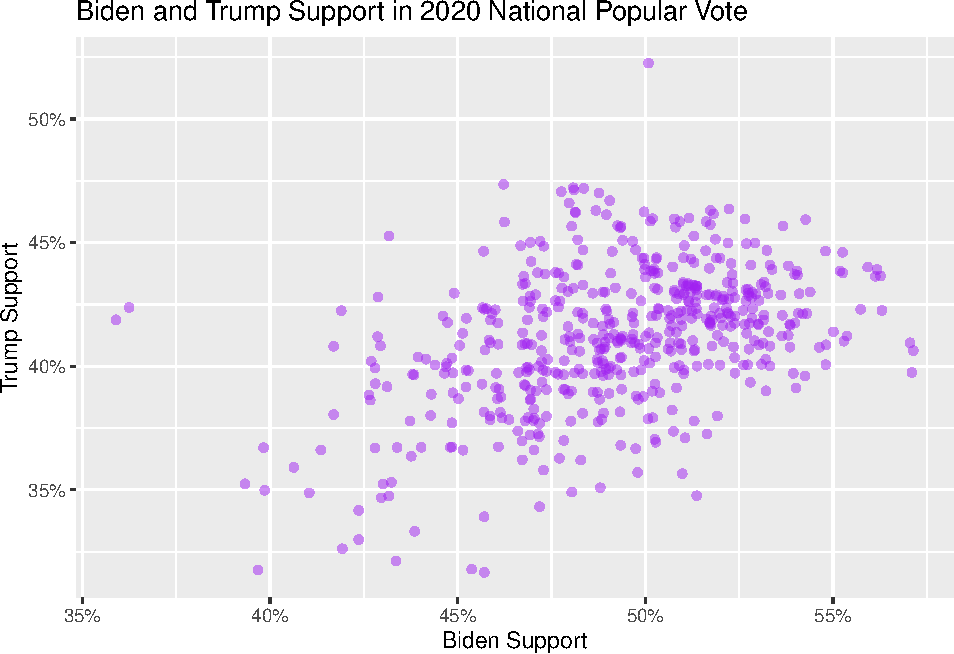
\includegraphics{psc4175_hw_8_files/figure-latex/unnamed-chunk-2-1.pdf}

What is an alternative explanation for these patterns? Why would polls
underpredict \emph{both} Trump and Biden?

Perhaps they were fielded earlier in the year, when more people were
interested in third party candidates, or hadn't made up their mind.

\section{Visualizing More Dimensions -- And Introducing
Dates!}\label{visualizing-more-dimensions-and-introducing-dates}

How did the support for Biden and Trump vary across the course of the
2020 Election?

\begin{itemize}
\item
  What should we measure?
\item
  How do we summarize, visualize, and communicate?
\end{itemize}

Give you some tools to do some \emph{amazing} things!

\section{Telling Time}\label{telling-time}

\begin{itemize}
\item
  Time is often a critical \emph{descriptive} variable. (Not causal!)
\item
  Also useful for \emph{prediction} ?
\item
  We want to evaluate the properties of presidential polling as Election
  Day 2020 approached.
\item
  Necessary for prediction -- we want most recent data to account for
  last-minute shift.
\item
  Necessary for identifying when changes occurred (and why?)
\end{itemize}

\section{Dates in R}\label{dates-in-r}

\begin{itemize}
\tightlist
\item
  Dates are a special format in R (character with quasi-numeric
  properties)
\end{itemize}

\begin{Shaded}
\begin{Highlighting}[]
\NormalTok{election.day }\OtherTok{\textless{}{-}} \FunctionTok{as.Date}\NormalTok{(}\StringTok{"11/3/2020"}\NormalTok{, }\StringTok{"\%m/\%d/\%Y"}\NormalTok{)   }
\NormalTok{election.day16 }\OtherTok{\textless{}{-}} \FunctionTok{as.Date}\NormalTok{(}\StringTok{"11/8/2016"}\NormalTok{, }\StringTok{"\%m/\%d/\%Y"}\NormalTok{)   }
\end{Highlighting}
\end{Shaded}

\begin{itemize}
\tightlist
\item
  Difference in ``dates'' versus difference in integers?
\end{itemize}

\begin{Shaded}
\begin{Highlighting}[]
\NormalTok{election.day }\SpecialCharTok{{-}}\NormalTok{ election.day16}
\end{Highlighting}
\end{Shaded}

\begin{verbatim}
## Time difference of 1456 days
\end{verbatim}

\begin{Shaded}
\begin{Highlighting}[]
\FunctionTok{as.numeric}\NormalTok{(election.day }\SpecialCharTok{{-}}\NormalTok{ election.day16)}
\end{Highlighting}
\end{Shaded}

\begin{verbatim}
## [1] 1456
\end{verbatim}

\section{Initial Questions}\label{initial-questions}

\begin{itemize}
\item
  How many polls were publicly done and reported in the media about the
  national popular vote?
\item
  When did the polling occur? Did most of the polls occur close to
  Election Day?
\end{itemize}

So, for every day, how many polls were reported by the media?

Note that we could also look to see if the poll results depend on how
the poll is being done (i.e., the \texttt{Mode} used to contact
respondents) or even depending on who funded (\texttt{Funded}) or
conducted (\texttt{Conducted}) the polls. We could also see if larger
polls (i.e., polls with more respondents \texttt{SampleSize}) or polls
that took longer to conduct (\texttt{DaysInField}) were more or less
accurate.

\section{Let's Wrangle\ldots{}}\label{lets-wrangle}

\begin{Shaded}
\begin{Highlighting}[]
\NormalTok{Pres2020.PV }\OtherTok{\textless{}{-}}\NormalTok{ Pres2020.PV }\SpecialCharTok{\%\textgreater{}\%}
                \FunctionTok{mutate}\NormalTok{(}\AttributeTok{EndDate =} \FunctionTok{as.Date}\NormalTok{(EndDate, }\StringTok{"\%m/\%d/\%Y"}\NormalTok{), }
                      \AttributeTok{StartDate =} \FunctionTok{as.Date}\NormalTok{(StartDate, }\StringTok{"\%m/\%d/\%Y"}\NormalTok{),}
                      \AttributeTok{DaysToED =} \FunctionTok{as.numeric}\NormalTok{(election.day }\SpecialCharTok{{-}}\NormalTok{ EndDate),}
                      \AttributeTok{Trump =}\NormalTok{ Trump}\SpecialCharTok{/}\DecValTok{100}\NormalTok{,}
                      \AttributeTok{Biden =}\NormalTok{ Biden}\SpecialCharTok{/}\DecValTok{100}\NormalTok{,}
                      \AttributeTok{margin =}\NormalTok{ Biden }\SpecialCharTok{{-}}\NormalTok{ Trump)}
\end{Highlighting}
\end{Shaded}

\section{What are we plotting?}\label{what-are-we-plotting}

\begin{itemize}
\item
  Media Question: how does the number of polls change over time?
\item
  Data Scientist Question: What do we need to plot? \texttt{margin} or
  \texttt{DaysToED}?
\item
  What will each produce?
\item
  Are they \emph{discrete/categorical} (barplot) or \emph{continuous}
  (histogram)?
\end{itemize}

\begin{Shaded}
\begin{Highlighting}[]
\FunctionTok{ggplot}\NormalTok{(}\AttributeTok{data =}\NormalTok{ Pres2020.PV, }\FunctionTok{aes}\NormalTok{(}\AttributeTok{x =}\NormalTok{ DaysToED)) }\SpecialCharTok{+}
  \FunctionTok{labs}\NormalTok{(}\AttributeTok{title =} \StringTok{"Number of 2020 National Polls Over Time"}\NormalTok{,}
       \AttributeTok{x =} \StringTok{"Number of Days until Election Day"}\NormalTok{,}
       \AttributeTok{y =} \StringTok{"Number of Polls"}\NormalTok{) }\SpecialCharTok{+} 
  \FunctionTok{geom\_bar}\NormalTok{(}\AttributeTok{fill=}\StringTok{"purple"}\NormalTok{, }\AttributeTok{color=} \StringTok{"black"}\NormalTok{) }\SpecialCharTok{+}
  \FunctionTok{scale\_x\_continuous}\NormalTok{(}\AttributeTok{breaks=}\FunctionTok{seq}\NormalTok{(}\DecValTok{0}\NormalTok{,}\DecValTok{230}\NormalTok{,}\AttributeTok{by=}\DecValTok{10}\NormalTok{)) }\SpecialCharTok{+}
  \FunctionTok{scale\_y\_continuous}\NormalTok{(}\AttributeTok{labels =} \FunctionTok{label\_number}\NormalTok{(}\AttributeTok{accuracy =} \DecValTok{1}\NormalTok{))}
\end{Highlighting}
\end{Shaded}

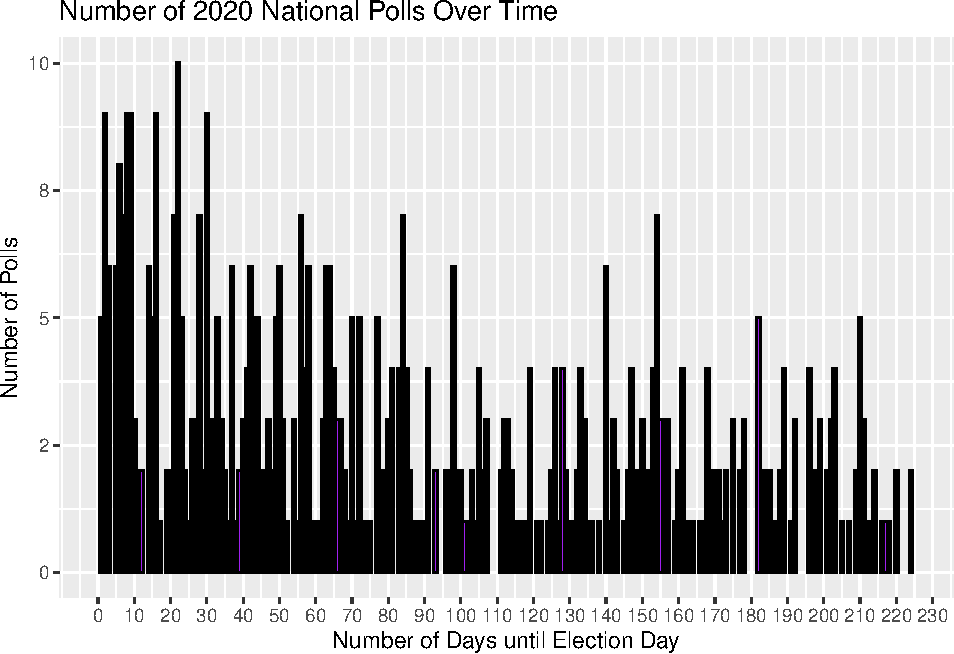
\includegraphics{psc4175_hw_8_files/figure-latex/unnamed-chunk-6-1.pdf}

So this is a bit weird because it arranges the axis from smallest to
largest even though that is in reverse chronological order. Since
November comes after January it may make sense to flip the scale so that
the graph plots polls that are closer to Election Day as the reader
moves along the scale to the left.

\begin{Shaded}
\begin{Highlighting}[]
\FunctionTok{ggplot}\NormalTok{(}\AttributeTok{data =}\NormalTok{ Pres2020.PV, }\FunctionTok{aes}\NormalTok{(}\AttributeTok{x =}\NormalTok{ DaysToED)) }\SpecialCharTok{+}
  \FunctionTok{labs}\NormalTok{(}\AttributeTok{title =} \StringTok{"Number of 2020 National Polls Over Time"}\NormalTok{) }\SpecialCharTok{+} 
  \FunctionTok{labs}\NormalTok{(}\AttributeTok{x =} \StringTok{"Number of Days until Election Day"}\NormalTok{) }\SpecialCharTok{+} 
  \FunctionTok{labs}\NormalTok{(}\AttributeTok{y =} \StringTok{"Number of Polls"}\NormalTok{) }\SpecialCharTok{+} 
  \FunctionTok{geom\_bar}\NormalTok{(}\AttributeTok{fill=}\StringTok{"purple"}\NormalTok{, }\AttributeTok{color=} \StringTok{"black"}\NormalTok{) }\SpecialCharTok{+}
  \FunctionTok{scale\_x\_reverse}\NormalTok{(}\AttributeTok{breaks=}\FunctionTok{seq}\NormalTok{(}\DecValTok{0}\NormalTok{,}\DecValTok{230}\NormalTok{,}\AttributeTok{by=}\DecValTok{10}\NormalTok{)) }\SpecialCharTok{+}
  \FunctionTok{scale\_y\_continuous}\NormalTok{(}\AttributeTok{labels =} \FunctionTok{label\_number}\NormalTok{(}\AttributeTok{accuracy =} \DecValTok{1}\NormalTok{))}
\end{Highlighting}
\end{Shaded}

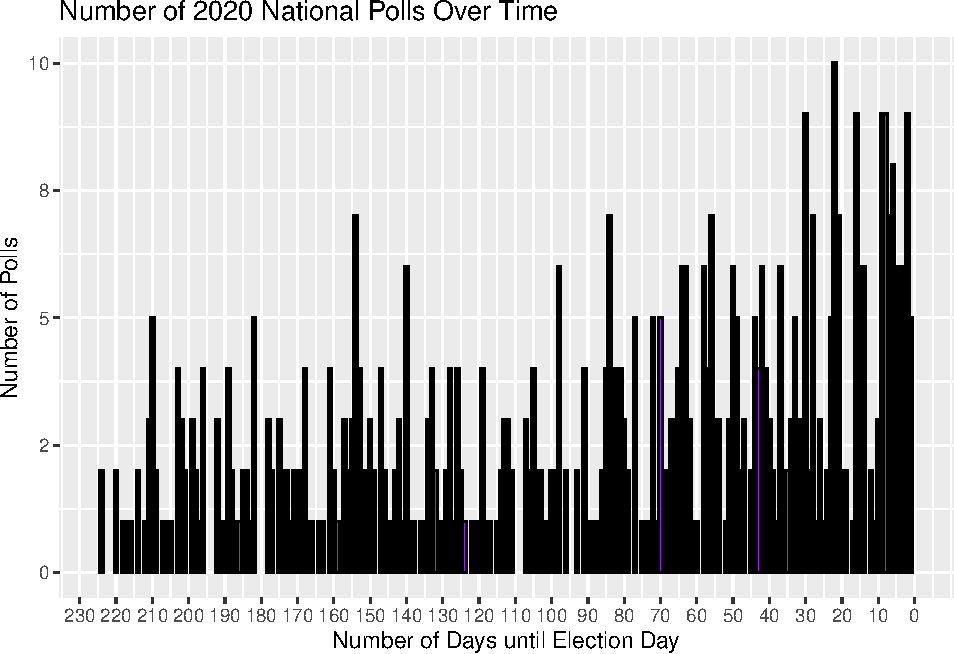
\includegraphics{psc4175_hw_8_files/figure-latex/unnamed-chunk-7-1.pdf}

But is the bargraph the right plot to use? Should we plot every single
day given that we know some days might contain fewer polls (e.g.,
weekends)? What if we to use a histogram instead to plot the number of
polls that occur in a set interval of time (to be defined by the number
of bins chosen)?

\begin{Shaded}
\begin{Highlighting}[]
\FunctionTok{ggplot}\NormalTok{(}\AttributeTok{data =}\NormalTok{ Pres2020.PV, }\FunctionTok{aes}\NormalTok{(}\AttributeTok{x =}\NormalTok{ DaysToED)) }\SpecialCharTok{+}
  \FunctionTok{labs}\NormalTok{(}\AttributeTok{title =} \StringTok{"Number of 2020 National Polls Over Time"}\NormalTok{) }\SpecialCharTok{+} 
  \FunctionTok{labs}\NormalTok{(}\AttributeTok{x =} \StringTok{"Number of Days until Election Day"}\NormalTok{) }\SpecialCharTok{+} 
  \FunctionTok{labs}\NormalTok{(}\AttributeTok{y =} \StringTok{"Number of Polls"}\NormalTok{) }\SpecialCharTok{+} 
  \FunctionTok{geom\_histogram}\NormalTok{(}\AttributeTok{color=}\StringTok{"PURPLE"}\NormalTok{,}\AttributeTok{bins =} \DecValTok{30}\NormalTok{) }\SpecialCharTok{+}
  \FunctionTok{scale\_x\_reverse}\NormalTok{()}
\end{Highlighting}
\end{Shaded}

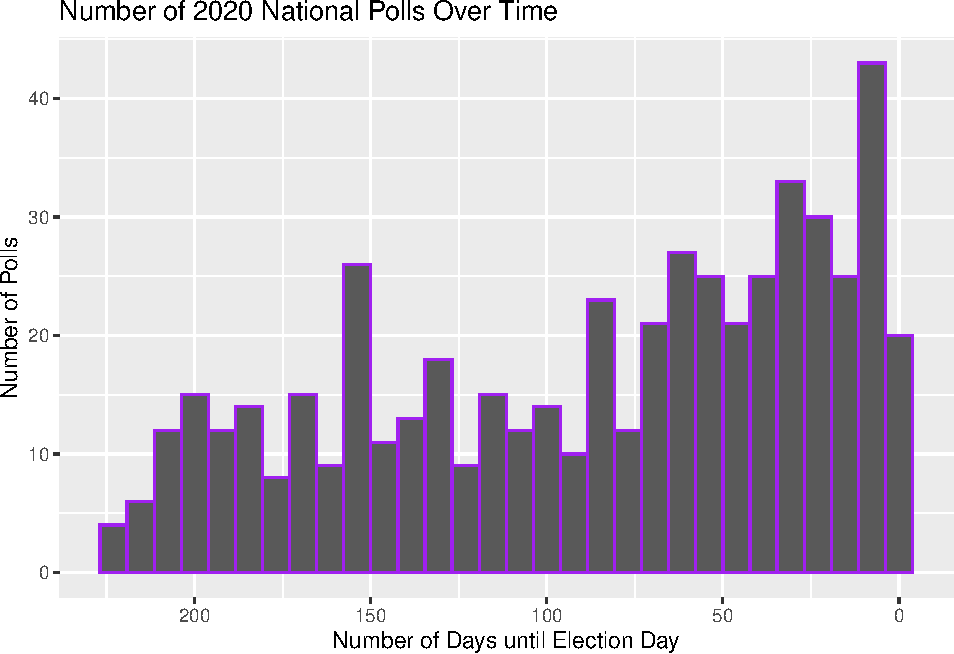
\includegraphics{psc4175_hw_8_files/figure-latex/unnamed-chunk-8-1.pdf}

Which do you prefer? Why or why not? Data Science is sometimes as much
art as it is science - especially when it comes to data visualization!

\section{Bivariate/Multivariate
relationships}\label{bivariatemultivariate-relationships}

\begin{itemize}
\item
  Most of what we do is a relationship between (at least) 2 variables.
\item
  Here we are interested in how the margin varies as Election Day
  approaches: \texttt{margin} by \texttt{DaysToED}.
\item
  Want to plot X (variable that ``explains'') vs.~Y (variable being
  ``explained''):
\end{itemize}

A very frequently used plot is the scatterplot that shows the
relationship between two variables. To do so we are going to define an
aesthetic when calling \texttt{ggplot} that defines both an x-variable
(here \texttt{EndDate}) and a y-variable (here \texttt{margin}).

First, a brief aside, we can change the size of the figure being printed
in our Rmarkdown by including some commands when defining the R chunk.
Much like we could suppress messages (e.g., \texttt{message=FALSE} or
tell R not to actually evaluate the chunk \texttt{eval=FALSE} or to run
the code but not print the code \texttt{echo=FALSE}) we can add some
arguments to this line. For example, the code below defines the figure
to be 2 inches tall, 2 inches wide and to be aligned in the center (as
opposed to left-justified). As you can see, depending on the choices you
make you can destroy the readability of the graphics as \texttt{ggplot}
will attempt to rescale the figure accordingly. The dimensions are in
inches and they refer to the plotting area -- an area that includes
labels and margins so it is \emph{not} the area where the data itself
appears.

\begin{Shaded}
\begin{Highlighting}[]
\NormalTok{margin\_over\_time\_plot }\OtherTok{\textless{}{-}}\NormalTok{ Pres2020.PV }\SpecialCharTok{\%\textgreater{}\%}
  \FunctionTok{ggplot}\NormalTok{(}\FunctionTok{aes}\NormalTok{(}\AttributeTok{x =}\NormalTok{ EndDate, }\AttributeTok{y =}\NormalTok{ margin)) }\SpecialCharTok{+} 
  \FunctionTok{labs}\NormalTok{(}\AttributeTok{title=}\StringTok{"Margin in 2020 National Popular Vote Polls Over Time"}\NormalTok{,}
       \AttributeTok{y =} \StringTok{"Margin: Biden {-} Trump"}\NormalTok{,}
       \AttributeTok{x =} \StringTok{"Poll Ending Date"}\NormalTok{) }\SpecialCharTok{+} 
  \FunctionTok{geom\_point}\NormalTok{(}\AttributeTok{color=}\StringTok{"purple"}\NormalTok{)}
\NormalTok{margin\_over\_time\_plot}
\end{Highlighting}
\end{Shaded}

\begin{center}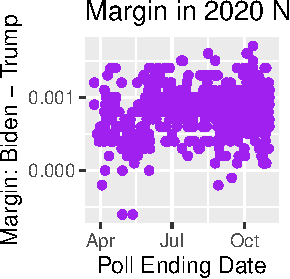
\includegraphics{psc4175_hw_8_files/figure-latex/unnamed-chunk-9-1} \end{center}

To ``fix'' this we can call the ggplot object without defining the
graphical parameters.

\begin{Shaded}
\begin{Highlighting}[]
\NormalTok{margin\_over\_time\_plot}
\end{Highlighting}
\end{Shaded}

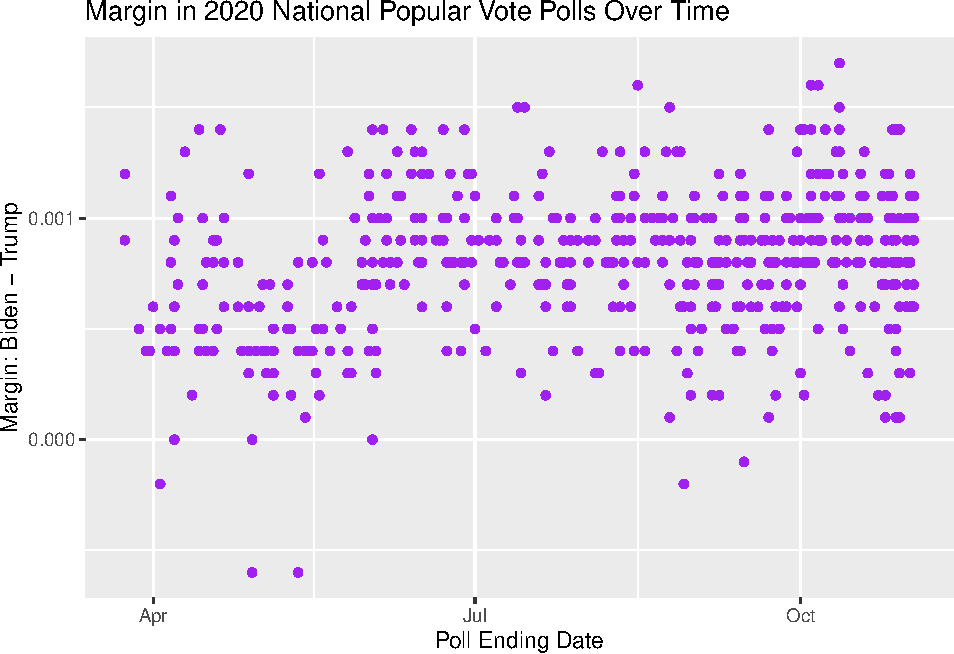
\includegraphics{psc4175_hw_8_files/figure-latex/unnamed-chunk-10-1.pdf}

Ok, back to fixing the graph. What do you think?

\begin{enumerate}
\def\labelenumi{\arabic{enumi}.}
\item
  Axes looks weird - lots of interpolation required by the consumer.
\item
  Data looks ``chunky''? How many data points are at each point?
\end{enumerate}

To fix the axis scale we can use \texttt{scale\_y\_continuous} to chose
better labels for the y-axis and we can use \texttt{scale\_x\_date} to
determine how to plot the dates we are plotting. Here we are going to
plot at two-week intervals (\texttt{date\_breaks\ =\ "2\ week"}) using
labels that include the month and date
(\texttt{date\_labels\ -\ "\%b\ \%d"}).

Note here that we are going to adjust the plot by adding new features to
the ggplot object \texttt{margin\_over\_time\_plot}. We could also have
created the graph without creating the object.

\begin{Shaded}
\begin{Highlighting}[]
\NormalTok{margin\_over\_time\_plot }\OtherTok{\textless{}{-}}\NormalTok{ margin\_over\_time\_plot  }\SpecialCharTok{+} 
    \FunctionTok{scale\_y\_continuous}\NormalTok{(}\AttributeTok{breaks=}\FunctionTok{seq}\NormalTok{(}\SpecialCharTok{{-}}\NormalTok{.}\DecValTok{1}\NormalTok{,.}\DecValTok{2}\NormalTok{,}\AttributeTok{by=}\NormalTok{.}\DecValTok{05}\NormalTok{),}
                     \AttributeTok{labels=}\NormalTok{ scales}\SpecialCharTok{::}\FunctionTok{percent\_format}\NormalTok{(}\AttributeTok{accuracy =} \DecValTok{1}\NormalTok{)) }\SpecialCharTok{+}
    \FunctionTok{scale\_x\_date}\NormalTok{(}\AttributeTok{date\_breaks =} \StringTok{"2 week"}\NormalTok{, }\AttributeTok{date\_labels =} \StringTok{"\%b \%d"}\NormalTok{) }
\NormalTok{margin\_over\_time\_plot}
\end{Highlighting}
\end{Shaded}

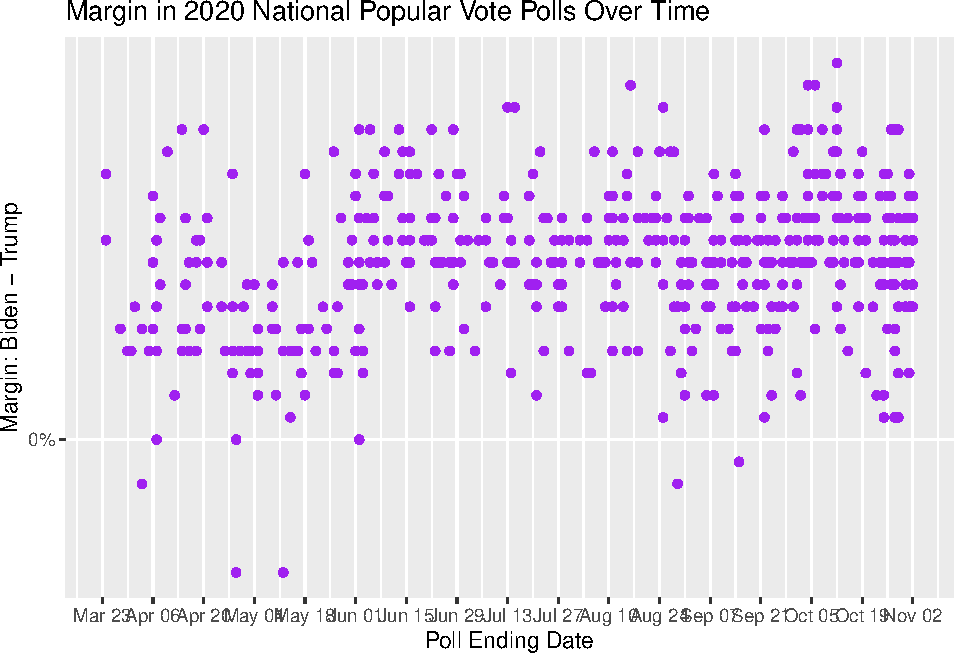
\includegraphics{psc4175_hw_8_files/figure-latex/unnamed-chunk-11-1.pdf}

Now one thing that is hard to know is how many polls are at a particular
point. If some points contain a single poll and others contain 1000
polls that matters a lot for how we interpret the relationship.

To help convey this information we can again use \texttt{geom\_jitter}
and alpha transparency instead of \texttt{geom\_point}. Here we are
adding +/- .005 to the y-value to change the value of the poll, but not
the date. (Note that we could also use \texttt{position=jitter} when
calling \texttt{geom\_point}). This adds just enough error in the x
(width) and y (height) values associated with each point so as to help
distinguish how many observations might share a value. We are also going
to use the alpha transparency to denote when lots of points occur on a
similar (jittered) point. Note that when doing this code we are going to
redo the plot from start to finish.

\begin{Shaded}
\begin{Highlighting}[]
\NormalTok{Pres2020.PV }\SpecialCharTok{\%\textgreater{}\%}
  \FunctionTok{ggplot}\NormalTok{(}\FunctionTok{aes}\NormalTok{(}\AttributeTok{x =}\NormalTok{ EndDate, }\AttributeTok{y =}\NormalTok{ margin)) }\SpecialCharTok{+} 
  \FunctionTok{labs}\NormalTok{(}\AttributeTok{title=}\StringTok{"Margin in 2020 National Popular Vote Polls Over Time"}\NormalTok{,}
       \AttributeTok{y =} \StringTok{"Margin: Biden {-} Trump"}\NormalTok{,}
       \AttributeTok{x =} \StringTok{"Poll Ending Date"}\NormalTok{) }\SpecialCharTok{+} 
    \FunctionTok{geom\_jitter}\NormalTok{(}\AttributeTok{color =} \StringTok{"PURPLE"}\NormalTok{,}\AttributeTok{height=}\NormalTok{.}\DecValTok{005}\NormalTok{, }\AttributeTok{alpha =}\NormalTok{ .}\DecValTok{4}\NormalTok{) }\SpecialCharTok{+}
    \FunctionTok{scale\_y\_continuous}\NormalTok{(}\AttributeTok{breaks=}\FunctionTok{seq}\NormalTok{(}\SpecialCharTok{{-}}\NormalTok{.}\DecValTok{1}\NormalTok{,.}\DecValTok{2}\NormalTok{,}\AttributeTok{by=}\NormalTok{.}\DecValTok{05}\NormalTok{),}
                     \AttributeTok{labels=}\NormalTok{ scales}\SpecialCharTok{::}\FunctionTok{percent\_format}\NormalTok{(}\AttributeTok{accuracy =} \DecValTok{1}\NormalTok{)) }\SpecialCharTok{+}
    \FunctionTok{scale\_x\_date}\NormalTok{(}\AttributeTok{date\_breaks =} \StringTok{"2 week"}\NormalTok{, }\AttributeTok{date\_labels =} \StringTok{"\%b \%d"}\NormalTok{) }
\end{Highlighting}
\end{Shaded}

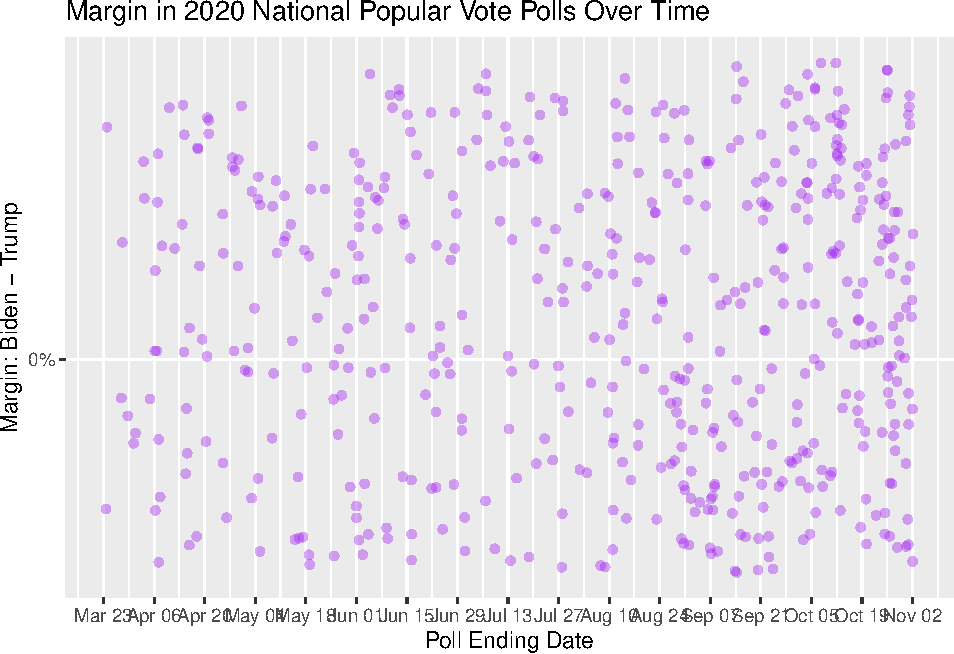
\includegraphics{psc4175_hw_8_files/figure-latex/unnamed-chunk-12-1.pdf}

In addition to plotting plotting points using \texttt{geom\_point} we
can also add lines to the plot using \texttt{geom\_line}. The line will
connect the values in sequence so it does not always make sense to
include. For example, if we add the \texttt{geom\_line} to the plot it
is hard to make the case that the results are meaningful.

\begin{Shaded}
\begin{Highlighting}[]
\NormalTok{Pres2020.PV }\SpecialCharTok{\%\textgreater{}\%}
  \FunctionTok{ggplot}\NormalTok{(}\FunctionTok{aes}\NormalTok{(}\AttributeTok{x =}\NormalTok{ EndDate, }\AttributeTok{y =}\NormalTok{ margin)) }\SpecialCharTok{+} 
  \FunctionTok{labs}\NormalTok{(}\AttributeTok{title=}\StringTok{"Margin in 2020 National Popular Vote Polls Over Time"}\NormalTok{,}
       \AttributeTok{y =} \StringTok{"Margin: Biden {-} Trump"}\NormalTok{,}
       \AttributeTok{x =} \StringTok{"Poll Ending Date"}\NormalTok{) }\SpecialCharTok{+} 
    \FunctionTok{geom\_jitter}\NormalTok{(}\AttributeTok{color=}\StringTok{"purple"}\NormalTok{, }\AttributeTok{alpha =}\NormalTok{ .}\DecValTok{5}\NormalTok{) }\SpecialCharTok{+} 
    \FunctionTok{scale\_y\_continuous}\NormalTok{(}\AttributeTok{breaks=}\FunctionTok{seq}\NormalTok{(}\SpecialCharTok{{-}}\NormalTok{.}\DecValTok{1}\NormalTok{,.}\DecValTok{2}\NormalTok{,}\AttributeTok{by=}\NormalTok{.}\DecValTok{05}\NormalTok{),}
                     \AttributeTok{labels=}\NormalTok{ scales}\SpecialCharTok{::}\FunctionTok{percent\_format}\NormalTok{(}\AttributeTok{accuracy =} \DecValTok{1}\NormalTok{)) }\SpecialCharTok{+}
    \FunctionTok{scale\_x\_date}\NormalTok{(}\AttributeTok{date\_breaks =} \StringTok{"2 week"}\NormalTok{, }\AttributeTok{date\_labels =} \StringTok{"\%b \%d"}\NormalTok{) }\SpecialCharTok{+}
  \FunctionTok{geom\_line}\NormalTok{()}
\end{Highlighting}
\end{Shaded}

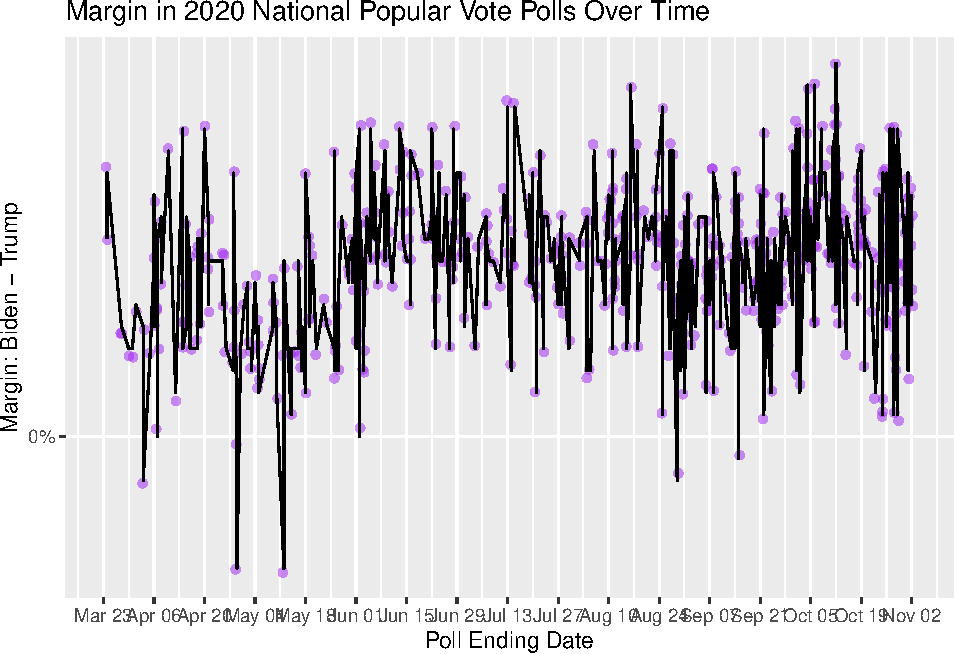
\includegraphics{psc4175_hw_8_files/figure-latex/unnamed-chunk-13-1.pdf}

While \texttt{geom\_line} may help accentuate variation over time, it is
really not designed to summarize a relationship in the data as it is
simply connecting sequential points (arranged according to the x-axis).
In contrast, if we were to add \texttt{geom\_smooth} then the plot would
add the average value of nearby points to help summarize the trend.
(Note that we have opted to include the associated uncertainty in the
moving average off using the \texttt{se=T} parameter in
\texttt{geom\_smooth}.)

\begin{Shaded}
\begin{Highlighting}[]
\CommentTok{\# Using message=FALSE to suppress note about geom\_smooth}
\NormalTok{Pres2020.PV }\SpecialCharTok{\%\textgreater{}\%}
  \FunctionTok{ggplot}\NormalTok{(}\FunctionTok{aes}\NormalTok{(}\AttributeTok{x =}\NormalTok{ EndDate, }\AttributeTok{y =}\NormalTok{ margin)) }\SpecialCharTok{+} 
  \FunctionTok{labs}\NormalTok{(}\AttributeTok{title=}\StringTok{"Margin in 2020 National Popular Vote Polls Over Time"}\NormalTok{,}
       \AttributeTok{y =} \StringTok{"Margin: Biden {-} Trump"}\NormalTok{,}
       \AttributeTok{x =} \StringTok{"Poll Ending Date"}\NormalTok{) }\SpecialCharTok{+} 
    \FunctionTok{geom\_jitter}\NormalTok{(}\AttributeTok{color=}\StringTok{"purple"}\NormalTok{, }\AttributeTok{alpha =}\NormalTok{ .}\DecValTok{5}\NormalTok{) }\SpecialCharTok{+} 
    \FunctionTok{scale\_y\_continuous}\NormalTok{(}\AttributeTok{breaks=}\FunctionTok{seq}\NormalTok{(}\SpecialCharTok{{-}}\NormalTok{.}\DecValTok{1}\NormalTok{,.}\DecValTok{2}\NormalTok{,}\AttributeTok{by=}\NormalTok{.}\DecValTok{05}\NormalTok{),}
                     \AttributeTok{labels=}\NormalTok{ scales}\SpecialCharTok{::}\FunctionTok{percent\_format}\NormalTok{(}\AttributeTok{accuracy =} \DecValTok{1}\NormalTok{)) }\SpecialCharTok{+}
    \FunctionTok{scale\_x\_date}\NormalTok{(}\AttributeTok{date\_breaks =} \StringTok{"2 week"}\NormalTok{, }\AttributeTok{date\_labels =} \StringTok{"\%b \%d"}\NormalTok{) }\SpecialCharTok{+}
    \FunctionTok{geom\_smooth}\NormalTok{(}\AttributeTok{color =} \StringTok{"BLACK"}\NormalTok{, }\AttributeTok{se=}\NormalTok{T) }
\end{Highlighting}
\end{Shaded}

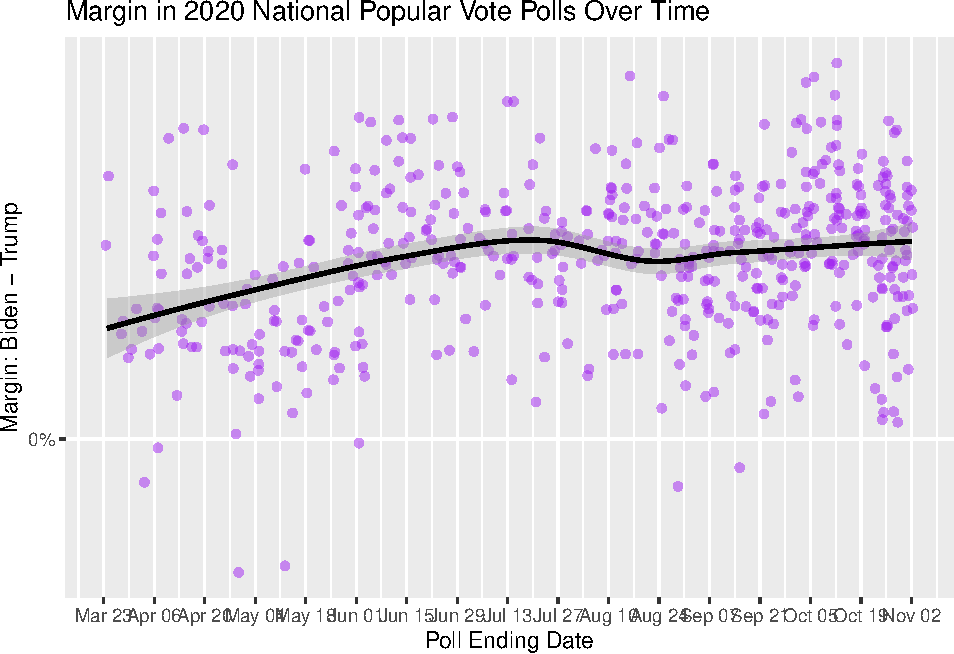
\includegraphics{psc4175_hw_8_files/figure-latex/unnamed-chunk-14-1.pdf}

\section{Plotting Multiple Variables Over Time
(Time-Series)}\label{plotting-multiple-variables-over-time-time-series}

\begin{itemize}
\tightlist
\item
  Can we plot support for Biden and support for Trump separately over
  time (on the same plot)?
\end{itemize}

Let's define a \texttt{ggplot} object to add to later. Note that this
code chuck will not print anything because we need to call the object to
see what it produced.

\begin{Shaded}
\begin{Highlighting}[]
\NormalTok{BidenTrumpplot }\OtherTok{\textless{}{-}}\NormalTok{ Pres2020.PV }\SpecialCharTok{\%\textgreater{}\%}
  \FunctionTok{ggplot}\NormalTok{()  }\SpecialCharTok{+}
  \FunctionTok{geom\_point}\NormalTok{(}\FunctionTok{aes}\NormalTok{(}\AttributeTok{x =}\NormalTok{ EndDate, }\AttributeTok{y =}\NormalTok{ Trump), }
             \AttributeTok{color =} \StringTok{"red"}\NormalTok{, }\AttributeTok{alpha=}\NormalTok{.}\DecValTok{4}\NormalTok{)  }\SpecialCharTok{+}
  \FunctionTok{geom\_point}\NormalTok{(}\FunctionTok{aes}\NormalTok{(}\AttributeTok{x =}\NormalTok{ EndDate, }\AttributeTok{y =}\NormalTok{ Biden), }
             \AttributeTok{color =} \StringTok{"blue"}\NormalTok{, }\AttributeTok{alpha=}\NormalTok{.}\DecValTok{4}\NormalTok{) }\SpecialCharTok{+}
  \FunctionTok{labs}\NormalTok{(}\AttributeTok{title=}\StringTok{"\% Biden and Trump in 2020 National Popular Vote Polls Over Time"}\NormalTok{,}
       \AttributeTok{y =} \StringTok{"Pct. Support"}\NormalTok{,}
       \AttributeTok{x =} \StringTok{"Poll Ending Date"}\NormalTok{) }\SpecialCharTok{+}
  \FunctionTok{scale\_x\_date}\NormalTok{(}\AttributeTok{date\_breaks =} \StringTok{"2 week"}\NormalTok{, }\AttributeTok{date\_labels =} \StringTok{"\%b \%d"}\NormalTok{) }\SpecialCharTok{+} 
  \FunctionTok{scale\_y\_continuous}\NormalTok{(}\AttributeTok{breaks=}\FunctionTok{seq}\NormalTok{(.}\DecValTok{3}\NormalTok{,.}\DecValTok{7}\NormalTok{,}\AttributeTok{by=}\NormalTok{.}\DecValTok{05}\NormalTok{),}
                     \AttributeTok{labels=}\NormalTok{ scales}\SpecialCharTok{::}\FunctionTok{percent\_format}\NormalTok{(}\AttributeTok{accuracy =} \DecValTok{1}\NormalTok{)) }
\end{Highlighting}
\end{Shaded}

\begin{itemize}
\tightlist
\item
  Note the use of \texttt{aes} in \texttt{geom\_point()}!
\end{itemize}

Now call the plot

\begin{Shaded}
\begin{Highlighting}[]
\NormalTok{BidenTrumpplot}
\end{Highlighting}
\end{Shaded}

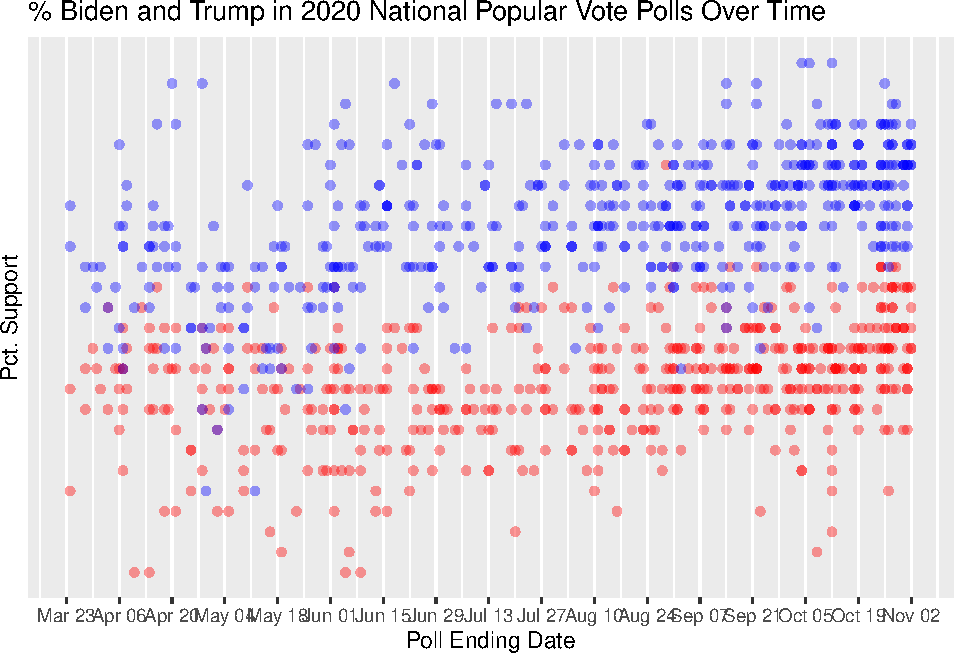
\includegraphics{psc4175_hw_8_files/figure-latex/unnamed-chunk-16-1.pdf}

Now we are going to add smoothed lines to the ggplot object. The nice
thing about having saved the ggplot object above is that to add the
smoothed lines we can simply add it to the existing plot.
\texttt{geom\_smooth} summarizes the average using a subset of the data
(the default is 75\%) by computing the average value for the closest
75\% of the data. Put differently, after sorting the polls by their date
it then summarizes the predicted value for a poll taken at that date
using the closest 75\% of polls according to the date. (It is not taking
a mean of those values, but it is doing something similar.) After doing
so for the first date, it then does the same for the second date, but
now the ``closest'' data includes polls that happened both before an
after. The smoother ``moves along'' the x-axis and generates a predicted
value for each date. Because it is using so much of the data, the values
of the line will change very slowly because the only change between two
adjacent dates is by dropping and adding new information.

When calling the \texttt{geom\_smooth} we used \texttt{se=T} to tell
\texttt{ggplot} to produce an estimate of how much the prediction may
vary. (This is the 95\% confidence interval for the prediction being
graphed.)

\begin{Shaded}
\begin{Highlighting}[]
\CommentTok{\# Using message=FALSE to suppress note about geom\_smooth}
\NormalTok{BidenTrumpplot }\SpecialCharTok{+}  
  \FunctionTok{geom\_smooth}\NormalTok{(}\FunctionTok{aes}\NormalTok{(}\AttributeTok{x =}\NormalTok{ EndDate, }\AttributeTok{y =}\NormalTok{ Trump), }
              \AttributeTok{color =} \StringTok{"red"}\NormalTok{,}\AttributeTok{se=}\NormalTok{T) }\SpecialCharTok{+} 
  \FunctionTok{geom\_smooth}\NormalTok{(}\FunctionTok{aes}\NormalTok{(}\AttributeTok{x =}\NormalTok{ EndDate, }\AttributeTok{y =}\NormalTok{ Biden), }
              \AttributeTok{color =} \StringTok{"blue"}\NormalTok{,}\AttributeTok{se=}\NormalTok{T)}
\end{Highlighting}
\end{Shaded}

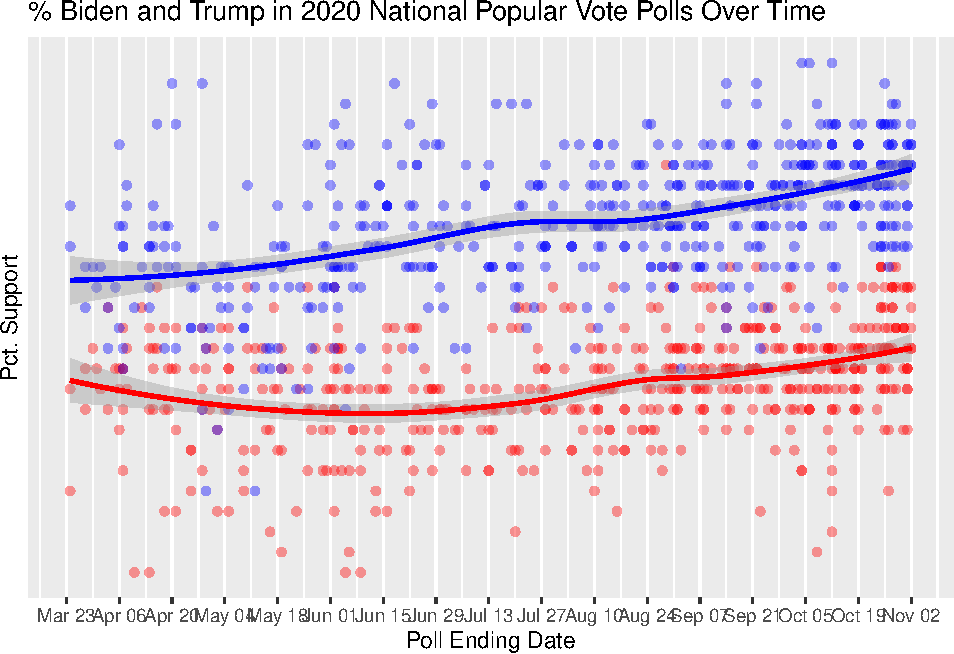
\includegraphics{psc4175_hw_8_files/figure-latex/unnamed-chunk-17-1.pdf}

If we change it to using only the closest 10\% of the data by changing
\texttt{span=.1} we get a slightly different relationship. The smoothed
lines are less smooth because the impact of adding and removing points
is much greater when we are using less data to compute the smoothed
value -- a single observation can change the overall results much more
than when we used so much more data. In addition, the error-bars around
the smoother are larger because we are using less data to calculate each
point.

\begin{Shaded}
\begin{Highlighting}[]
\CommentTok{\# Using message=FALSE to suppress note about geom\_smooth}
\NormalTok{BidenTrumpplot }\SpecialCharTok{+}  
  \FunctionTok{geom\_smooth}\NormalTok{(}\FunctionTok{aes}\NormalTok{(}\AttributeTok{x =}\NormalTok{ EndDate, }\AttributeTok{y =}\NormalTok{ Trump), }
              \AttributeTok{color =} \StringTok{"red"}\NormalTok{,}\AttributeTok{se=}\NormalTok{T,}\AttributeTok{span=}\NormalTok{.}\DecValTok{1}\NormalTok{) }\SpecialCharTok{+} 
  \FunctionTok{geom\_smooth}\NormalTok{(}\FunctionTok{aes}\NormalTok{(}\AttributeTok{x =}\NormalTok{ EndDate, }\AttributeTok{y =}\NormalTok{ Biden), }
              \AttributeTok{color =} \StringTok{"blue"}\NormalTok{,}\AttributeTok{se=}\NormalTok{T,}\AttributeTok{span=}\NormalTok{.}\DecValTok{1}\NormalTok{)}
\end{Highlighting}
\end{Shaded}

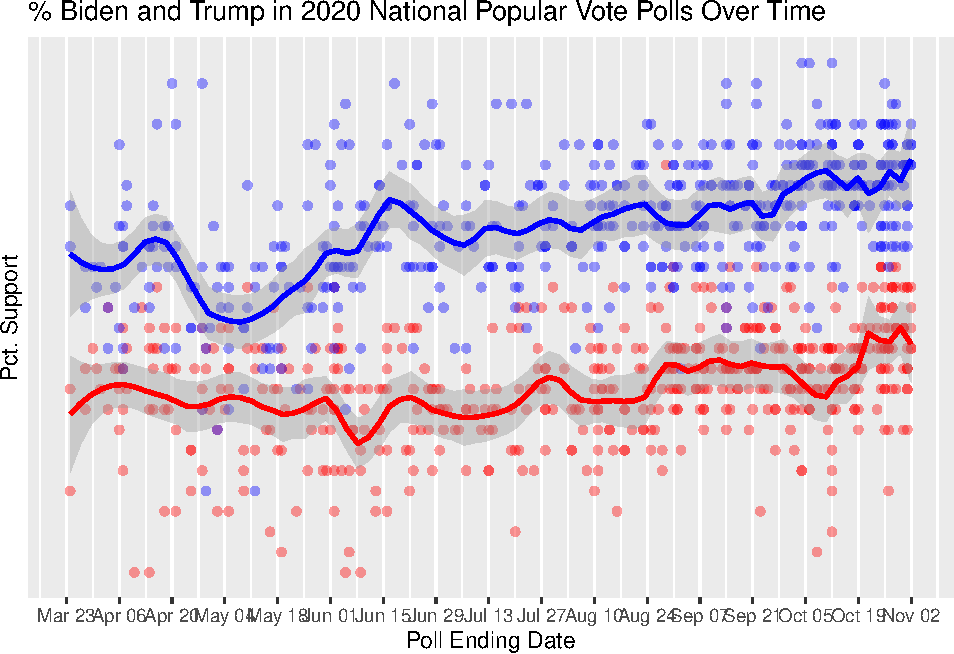
\includegraphics{psc4175_hw_8_files/figure-latex/unnamed-chunk-18-1.pdf}

Try some other values to see how things change. Note that you are not
changing the data, you are only changing how you are visualizing the
relationship over time by deciding how much data to use. In part, the
decision of how much data to use is a question of how much you you want
to allow public opinion to vary over the course of the campaign -- how
much of the variation is ``real'' versus how much is ``noise''?

\emph{Quick Exercise} Choose another span and see how it changes how you
interpret how much variation there is in the data over time.

\begin{Shaded}
\begin{Highlighting}[]
\CommentTok{\# INSERT CODE}
\end{Highlighting}
\end{Shaded}

\textbf{\emph{ADVANCED!}} We can also use \texttt{fill} to introduce
another dimension into the visualization. Consider for example, plotting
support for Trump over time for mixed-mode polls versus telephone polls
versus online-only polls. How would you go about doing this? You want to
be careful not to make a mess however. Just because you can doesn't mean
you should!

\section{State Polls and the Electoral
College}\label{state-polls-and-the-electoral-college}

New functions and libraries:

\begin{itemize}
\tightlist
\item
  \texttt{plotly} library
\item
  Working with dates
\item
  Simple looping
\end{itemize}

First load the data of all state-level polls for the 2020 presidential
election.

\begin{Shaded}
\begin{Highlighting}[]
\NormalTok{Pres2020.StatePolls }\OtherTok{\textless{}{-}} \FunctionTok{read\_rds}\NormalTok{(}\AttributeTok{file=}\StringTok{"https://github.com/rweldzius/PSC4175\_F2024/raw/main/Data/Pres2020\_StatePolls.Rds"}\NormalTok{)}
\FunctionTok{glimpse}\NormalTok{(Pres2020.StatePolls)}
\end{Highlighting}
\end{Shaded}

\begin{verbatim}
## Rows: 1,545
## Columns: 19
## $ StartDate      <date> 2020-03-21, 2020-03-24, 2020-03-24, 2020-03-28, 2020-0~
## $ EndDate        <date> 2020-03-30, 2020-04-03, 2020-03-29, 2020-03-29, 2020-0~
## $ DaysinField    <dbl> 10, 11, 6, 2, 3, 5, 2, 2, 7, 3, 3, 3, 2, 2, 3, 4, 10, 1~
## $ MoE            <dbl> 2.8, 3.0, 4.2, NA, 4.0, 1.7, 3.0, 3.1, 4.1, 4.4, NA, NA~
## $ Mode           <chr> "Phone/Online", "Phone/Online", "Live phone - RDD", "Li~
## $ SampleSize     <dbl> 1331, 1000, 813, 962, 602, 3244, 1035, 1019, 583, 500, ~
## $ Biden          <dbl> 41, 47, 48, 67, 46, 46, 46, 48, 52, 42, 48, 50, 52, 38,~
## $ Trump          <dbl> 46, 34, 45, 29, 46, 40, 48, 45, 39, 49, 47, 41, 43, 49,~
## $ Winner         <chr> "Rep", "Dem", "Dem", "Dem", "Dem", "Rep", "Dem", "Dem",~
## $ poll.predicted <dbl> 1, 1, 1, 1, 0, 0, 0, 1, 1, 1, 1, 1, 1, 1, 1, 1, 1, 1, 1~
## $ Funded         <chr> "UtahPolicy.com & KUTV 2News", "Sacred Heart University~
## $ Conducted      <chr> "Y2 Analytics", "GreatBlue Research", "LHK Partners Inc~
## $ margin         <dbl> -5, 13, 3, 38, 0, 6, -2, 3, 13, -7, 1, 9, 9, -11, 6, -1~
## $ DaysToED       <drtn> 218 days, 214 days, 219 days, 219 days, 216 days, 213 ~
## $ StateName      <chr> "Utah", "Connecticut", "Wisconsin", "California", "Mich~
## $ EV             <int> 6, 7, 10, 55, 16, 29, 16, 16, 12, 15, 10, 16, 11, 6, 16~
## $ State          <chr> "UT", "CT", "WI", "CA", "MI", "FL", "GA", "MI", "WA", "~
## $ BidenCertVote  <dbl> 38, 59, 49, 64, 51, 48, 50, 51, 58, 49, 49, 51, 49, 41,~
## $ TrumpCertVote  <dbl> 58, 39, 49, 34, 48, 51, 49, 48, 39, 50, 49, 48, 49, 58,~
\end{verbatim}

Variables of potential interest include:

\begin{itemize}
\tightlist
\item
  \emph{Biden} : Percentage of respondents supporting Biden, the
  Democrat, in poll (0-100)
\item
  \emph{Trump} : Percentage of respondents supporting Trump, the
  Republican, in poll (0-100)
\item
  \emph{BidenCertVote} : Percentage of vote Biden, the Democrat,
  actually received in the election (0-100)
\item
  \emph{TrumpCertVote} : Percentage of vote Trump, the Democrat,
  actually received in the election (0-100)
\item
  \emph{Winner} : whether Biden won (``Dem'') or Trump won (``Rep'')
\item
  \emph{poll.predicted} : Indicator for whether the poll correctly
  predicted who won (1) or not (0)
\item
  \emph{State} \& \emph{StateName} : the state where the poll was
  conducted
\item
  \emph{EV} : the number of Electoral College Votes the state is worth
  for the winning candidate
\end{itemize}

\section{Overall Task:}\label{overall-task}

\begin{itemize}
\tightlist
\item
  How do we use this data to calculate the probability that Biden will
  win the presidency of the United States by winning the Electoral
  College?
\end{itemize}

\subsubsection{Task 1: How should we translate a poll result into a
predicted
probability?}\label{task-1-how-should-we-translate-a-poll-result-into-a-predicted-probability}

Suppose that I give you 10 polls from a state.

Load in the data and create the some mutations to create new variables.

\begin{Shaded}
\begin{Highlighting}[]
\NormalTok{Pres2020.StatePolls }\OtherTok{\textless{}{-}}\NormalTok{ Pres2020.StatePolls }\SpecialCharTok{\%\textgreater{}\%}
   \FunctionTok{mutate}\NormalTok{(}\AttributeTok{BidenNorm =}\NormalTok{ Biden}\SpecialCharTok{/}\NormalTok{(Biden}\SpecialCharTok{+}\NormalTok{Trump),}
          \AttributeTok{TrumpNorm =} \DecValTok{1}\SpecialCharTok{{-}}\NormalTok{BidenNorm,}
          \AttributeTok{Biden =}\NormalTok{ Biden}\SpecialCharTok{/}\DecValTok{100}\NormalTok{,}
          \AttributeTok{Trump=}\NormalTok{Trump}\SpecialCharTok{/}\DecValTok{100}\NormalTok{)}
\end{Highlighting}
\end{Shaded}

How can you use them to create a probability? Discuss! (I can think of 3
ways.)

\begin{itemize}
\tightlist
\item
  Measure 1: Fraction of polls with Biden in the lead
\item
  Measure 2: Biden Pct = Probability Biden wins
\item
  Measure 3: Normalized Biden Pct = Probability Biden wins (i.e., all
  voters either vote for Biden or Trump). Sometimes called ``two-party''
  vote.
\end{itemize}

How does this vary across states? The joys of \texttt{group\_by()}. Note
that \texttt{group\_by()} defines what happens for all subsequent code
in that code chunk. So here we are going to calculate the mean
separately for each state.

\begin{Shaded}
\begin{Highlighting}[]
\NormalTok{stateprobs }\OtherTok{\textless{}{-}}\NormalTok{ Pres2020.StatePolls }\SpecialCharTok{\%\textgreater{}\%}
    \FunctionTok{group\_by}\NormalTok{(StateName) }\SpecialCharTok{\%\textgreater{}\%}
      \FunctionTok{summarize}\NormalTok{(}\AttributeTok{BidenProbWin1 =} \FunctionTok{mean}\NormalTok{(Biden }\SpecialCharTok{\textgreater{}}\NormalTok{ Trump),}
                \AttributeTok{BidenProbWin2 =} \FunctionTok{mean}\NormalTok{(Biden),  }
                \AttributeTok{BidenProbWin3 =} \FunctionTok{mean}\NormalTok{(BidenNorm))}

\NormalTok{stateprobs}
\end{Highlighting}
\end{Shaded}

\begin{verbatim}
## # A tibble: 50 x 4
##    StateName   BidenProbWin1 BidenProbWin2 BidenProbWin3
##    <chr>               <dbl>         <dbl>         <dbl>
##  1 Alabama             0             0.389         0.407
##  2 Alaska              0             0.442         0.466
##  3 Arizona             0.840         0.484         0.519
##  4 Arkansas            0             0.381         0.395
##  5 California          1             0.618         0.661
##  6 Colorado            1             0.534         0.571
##  7 Connecticut         1             0.584         0.631
##  8 Delaware            1             0.603         0.627
##  9 Florida             0.798         0.486         0.517
## 10 Georgia             0.548         0.474         0.504
## # i 40 more rows
\end{verbatim}

Clearly they differ, so let's visualize to try to understand what is
going on. Install the library \texttt{plotly}

\begin{Shaded}
\begin{Highlighting}[]
\FunctionTok{library}\NormalTok{(plotly)}
\NormalTok{gg }\OtherTok{\textless{}{-}}\NormalTok{ stateprobs }\SpecialCharTok{\%\textgreater{}\%}
  \FunctionTok{ggplot}\NormalTok{(}\FunctionTok{aes}\NormalTok{(}\AttributeTok{x=}\NormalTok{BidenProbWin2, }\AttributeTok{y=}\NormalTok{BidenProbWin3,}\AttributeTok{text=}\FunctionTok{paste}\NormalTok{(StateName))) }\SpecialCharTok{+}
  \FunctionTok{geom\_point}\NormalTok{() }\SpecialCharTok{+}
  \FunctionTok{geom\_abline}\NormalTok{(}\AttributeTok{intercept=}\DecValTok{0}\NormalTok{,}\AttributeTok{slope=}\DecValTok{1}\NormalTok{) }\SpecialCharTok{+}
  \FunctionTok{labs}\NormalTok{(}\AttributeTok{x=} \StringTok{"Probability as \% Support"}\NormalTok{,}
       \AttributeTok{y =} \StringTok{"Probability as Two{-}Party \% Support"}\NormalTok{,}
       \AttributeTok{title =} \StringTok{"Comparing Probability of Winning Measures"}\NormalTok{)}

\FunctionTok{ggplotly}\NormalTok{(gg,}\AttributeTok{tooltip =} \StringTok{"text"}\NormalTok{)}
\end{Highlighting}
\end{Shaded}

\includegraphics{psc4175_hw_8_files/figure-latex/unnamed-chunk-23-1.pdf}

So removing the undecided and making the probabilities for Biden and
Trump sum to 100\% is consequential.

What about if we compare these measures to the fration of polls with a
given winner? After all, it seems implausible that the Biden would ever
lose California or Trump would ever lose Tennessee.

\begin{Shaded}
\begin{Highlighting}[]
\FunctionTok{library}\NormalTok{(plotly)}
\NormalTok{gg }\OtherTok{\textless{}{-}}\NormalTok{ stateprobs }\SpecialCharTok{\%\textgreater{}\%}
  \FunctionTok{ggplot}\NormalTok{(}\FunctionTok{aes}\NormalTok{(}\AttributeTok{x=}\NormalTok{BidenProbWin2, }\AttributeTok{y=}\NormalTok{BidenProbWin1,}\AttributeTok{text=}\FunctionTok{paste}\NormalTok{(StateName))) }\SpecialCharTok{+}
  \FunctionTok{geom\_point}\NormalTok{() }\SpecialCharTok{+}
  \FunctionTok{geom\_abline}\NormalTok{(}\AttributeTok{intercept=}\DecValTok{0}\NormalTok{,}\AttributeTok{slope=}\DecValTok{1}\NormalTok{) }\SpecialCharTok{+}
  \FunctionTok{labs}\NormalTok{(}\AttributeTok{x=} \StringTok{"Probability as \% Support"}\NormalTok{,}
       \AttributeTok{y =} \StringTok{"Probability as \% Polls Winning"}\NormalTok{,}
       \AttributeTok{title =} \StringTok{"Comparing Probability of Winning Measures"}\NormalTok{)}

\FunctionTok{ggplotly}\NormalTok{(gg,}\AttributeTok{tooltip =} \StringTok{"text"}\NormalTok{)}
\end{Highlighting}
\end{Shaded}

\includegraphics{psc4175_hw_8_files/figure-latex/unnamed-chunk-24-1.pdf}

So what do you think? Exactly the same data, but just different
impications depending on how you choose to measure the probability of
winning a state. Data sciene is as much about argument and reasoning as
it is about coding. How we measure a concept is often critical to the
conclusions that we get.

\subsubsection{Task 2: Start ``simple'' -- calculate the probability
that Biden wins
PA}\label{task-2-start-simple-calculate-the-probability-that-biden-wins-pa}

But we want to combine these probabilities with the Electoral College
votes in each state. Not every state has the same amount of Electoral
College votes -- it is typically given by the number of Senators (2)
plus the number of representatives (at least 1) so we need to account
for this if we want to make a projection about who is going to win the
Electoral College.

\begin{itemize}
\tightlist
\item
  Create a tibble with just polls from PA.
\end{itemize}

\begin{Shaded}
\begin{Highlighting}[]
\NormalTok{PA.dat }\OtherTok{\textless{}{-}}\NormalTok{ Pres2020.StatePolls }\SpecialCharTok{\%\textgreater{}\%} 
  \FunctionTok{filter}\NormalTok{(State }\SpecialCharTok{==} \StringTok{"PA"}\NormalTok{)}
\end{Highlighting}
\end{Shaded}

\begin{itemize}
\tightlist
\item
  Now compute these three probabilities. What functions do we need?
\end{itemize}

\begin{Shaded}
\begin{Highlighting}[]
\NormalTok{PA.dat }\SpecialCharTok{\%\textgreater{}\%}
      \FunctionTok{summarize}\NormalTok{(}\AttributeTok{BidenProbWin1 =} \FunctionTok{mean}\NormalTok{(Biden }\SpecialCharTok{\textgreater{}}\NormalTok{ Trump),}
                \AttributeTok{BidenProbWin2 =} \FunctionTok{mean}\NormalTok{(Biden),  }
                \AttributeTok{BidenProbWin3 =} \FunctionTok{mean}\NormalTok{(BidenNorm))}
\end{Highlighting}
\end{Shaded}

\begin{verbatim}
## # A tibble: 1 x 3
##   BidenProbWin1 BidenProbWin2 BidenProbWin3
##           <dbl>         <dbl>         <dbl>
## 1         0.916         0.499         0.529
\end{verbatim}

\begin{itemize}
\tightlist
\item
  What do you think about this?
\end{itemize}

\subsubsection{\texorpdfstring{Task 3: Given that probability, how do we
change the code to compute the expected number of Electoral College
Votes \texttt{EV} for
Biden?}{Task 3: Given that probability, how do we change the code to compute the expected number of Electoral College Votes EV for Biden?}}\label{task-3-given-that-probability-how-do-we-change-the-code-to-compute-the-expected-number-of-electoral-college-votes-ev-for-biden}

\begin{itemize}
\tightlist
\item
  Keep the code from above and copy and paste so you can understand how
  each step changes what we are doing. Note that we have the number of
  electoral college votes associated with each state \texttt{EV} that we
  want to use to compute the expected number of electoral college votes.
  But recall that when we \texttt{summarize} we change the tibble to be
  the output of the function. So how do we keep the number of Electoral
  College votes for a future mutation?
\end{itemize}

\begin{Shaded}
\begin{Highlighting}[]
\NormalTok{PA.dat }\SpecialCharTok{\%\textgreater{}\%}
      \FunctionTok{summarize}\NormalTok{(}\AttributeTok{BidenProbWin1 =} \FunctionTok{mean}\NormalTok{(Biden }\SpecialCharTok{\textgreater{}}\NormalTok{ Trump),}
                \AttributeTok{BidenProbWin2 =} \FunctionTok{mean}\NormalTok{(Biden),}
                \AttributeTok{BidenProbWin3 =} \FunctionTok{mean}\NormalTok{(BidenNorm),}
                \AttributeTok{EV =} \FunctionTok{mean}\NormalTok{(EV)) }\SpecialCharTok{\%\textgreater{}\%}
      \FunctionTok{mutate}\NormalTok{(}\AttributeTok{BidenEV1 =}\NormalTok{ BidenProbWin1}\SpecialCharTok{*}\NormalTok{EV,}
             \AttributeTok{BidenEV2 =}\NormalTok{ BidenProbWin2}\SpecialCharTok{*}\NormalTok{EV,}
             \AttributeTok{BidenEV3 =}\NormalTok{ BidenProbWin3}\SpecialCharTok{*}\NormalTok{EV)}
\end{Highlighting}
\end{Shaded}

\begin{verbatim}
## # A tibble: 1 x 7
##   BidenProbWin1 BidenProbWin2 BidenProbWin3    EV BidenEV1 BidenEV2 BidenEV3
##           <dbl>         <dbl>         <dbl> <dbl>    <dbl>    <dbl>    <dbl>
## 1         0.916         0.499         0.529    20     18.3     9.98     10.6
\end{verbatim}

Note that we are calculation the Expected Value of the Electoral College
votes using: \emph{Probability that Biden wins state i} X
\emph{Electoral College Votes in State i}. This will allocate fractions
of Electoral College votes even though the actual election is
winner-take all. This is OK because the fractions reflect the
probability that an alternative outcome occurs.

\emph{Quick Exercise} How can we get compute the expected number of
Electoral College votes for Trump in each measure? NOTE: There are at
least 2 ways to do this because this is a 2 candidate race

\begin{Shaded}
\begin{Highlighting}[]
\CommentTok{\# INSERT CODE HERE}
\end{Highlighting}
\end{Shaded}

\begin{itemize}
\tightlist
\item
  \texttt{EV-BidenEV}, or compute \texttt{TrumpProbWin}
\end{itemize}

\subsubsection{Task 4: Now generalize to every state by applying this
code to each set of state
polls.}\label{task-4-now-generalize-to-every-state-by-applying-this-code-to-each-set-of-state-polls.}

\begin{itemize}
\tightlist
\item
  What do we need to do this calculation for every state in our tibble?
\item
  First, compute probability of winning a state. (How?)
\item
  Second, compute expected Electoral College Votes. (How?)
\end{itemize}

\begin{Shaded}
\begin{Highlighting}[]
\NormalTok{Pres2020.StatePolls }\SpecialCharTok{\%\textgreater{}\%}  
  \FunctionTok{group\_by}\NormalTok{(StateName) }\SpecialCharTok{\%\textgreater{}\%}
    \FunctionTok{summarize}\NormalTok{(}\AttributeTok{BidenProbWin1 =} \FunctionTok{mean}\NormalTok{(Biden }\SpecialCharTok{\textgreater{}}\NormalTok{ Trump),}
              \AttributeTok{BidenProbWin3 =} \FunctionTok{mean}\NormalTok{(BidenNorm),}
              \AttributeTok{EV =} \FunctionTok{mean}\NormalTok{(EV),}
              \AttributeTok{State =} \FunctionTok{first}\NormalTok{(State)) }\SpecialCharTok{\%\textgreater{}\%}
    \FunctionTok{mutate}\NormalTok{(}\AttributeTok{State =}\NormalTok{ State,}
              \AttributeTok{BidenECVPredicted1 =}\NormalTok{ EV}\SpecialCharTok{*}\NormalTok{BidenProbWin1,}
              \AttributeTok{TrumpECVPredicted1 =}\NormalTok{ EV}\SpecialCharTok{{-}}\NormalTok{ BidenECVPredicted1,}
              \AttributeTok{BidenECVPredicted3 =}\NormalTok{ EV}\SpecialCharTok{*}\NormalTok{BidenProbWin3,}
              \AttributeTok{TrumpECVPredicted3 =}\NormalTok{ EV}\SpecialCharTok{{-}}\NormalTok{ BidenECVPredicted3) }\SpecialCharTok{\%\textgreater{}\%}
  \FunctionTok{summarize}\NormalTok{(}\AttributeTok{BidenECVPredicted1=}\FunctionTok{sum}\NormalTok{(BidenECVPredicted1),}
            \AttributeTok{BidenECVPredicted3=}\FunctionTok{sum}\NormalTok{(BidenECVPredicted3),}
            \AttributeTok{TrumpECVPredicted1=}\FunctionTok{sum}\NormalTok{(TrumpECVPredicted1),}
            \AttributeTok{TrumpECVPredicted3=}\FunctionTok{sum}\NormalTok{(TrumpECVPredicted3),)}
\end{Highlighting}
\end{Shaded}

\begin{verbatim}
## # A tibble: 1 x 4
##   BidenECVPredicted1 BidenECVPredicted3 TrumpECVPredicted1 TrumpECVPredicted3
##                <dbl>              <dbl>              <dbl>              <dbl>
## 1               345.               289.               190.               246.
\end{verbatim}

\subsubsection{Task 5: Now compute total expected vote by adding to that
code}\label{task-5-now-compute-total-expected-vote-by-adding-to-that-code}

\begin{itemize}
\tightlist
\item
  NOTE: Actually 306 - 232
\item
  What do we need to do to the tibble we created in Task 4 to get the
  overall number of Electoral College Votes?
\end{itemize}

\begin{Shaded}
\begin{Highlighting}[]
\NormalTok{Pres2020.StatePolls }\SpecialCharTok{\%\textgreater{}\%}  
  \FunctionTok{group\_by}\NormalTok{(StateName) }\SpecialCharTok{\%\textgreater{}\%}
    \FunctionTok{summarize}\NormalTok{(}\AttributeTok{BidenProbWin1 =} \FunctionTok{mean}\NormalTok{(Biden }\SpecialCharTok{\textgreater{}}\NormalTok{ Trump),}
              \AttributeTok{BidenProbWin3 =} \FunctionTok{mean}\NormalTok{(BidenNorm),}
              \AttributeTok{EV =} \FunctionTok{mean}\NormalTok{(EV)) }\SpecialCharTok{\%\textgreater{}\%}
    \FunctionTok{mutate}\NormalTok{(}\AttributeTok{BidenECVPredicted1 =}\NormalTok{ EV}\SpecialCharTok{*}\NormalTok{BidenProbWin1,}
              \AttributeTok{TrumpECVPredicted1 =}\NormalTok{ EV}\SpecialCharTok{{-}}\NormalTok{ BidenECVPredicted1,}
              \AttributeTok{BidenECVPredicted3 =}\NormalTok{ EV}\SpecialCharTok{*}\NormalTok{BidenProbWin3,}
              \AttributeTok{TrumpECVPredicted3 =}\NormalTok{ EV}\SpecialCharTok{{-}}\NormalTok{ BidenECVPredicted3) }\SpecialCharTok{\%\textgreater{}\%}
    \FunctionTok{summarize}\NormalTok{(}\AttributeTok{BidenECV1 =} \FunctionTok{sum}\NormalTok{(BidenECVPredicted1),}
              \AttributeTok{TrumpECV1 =} \FunctionTok{sum}\NormalTok{(TrumpECVPredicted1),}
              \AttributeTok{BidenECV3 =} \FunctionTok{sum}\NormalTok{(BidenECVPredicted3),}
              \AttributeTok{TrumpECV3 =} \FunctionTok{sum}\NormalTok{(TrumpECVPredicted3))}
\end{Highlighting}
\end{Shaded}

\begin{verbatim}
## # A tibble: 1 x 4
##   BidenECV1 TrumpECV1 BidenECV3 TrumpECV3
##       <dbl>     <dbl>     <dbl>     <dbl>
## 1      345.      190.      289.      246.
\end{verbatim}

\emph{Quick Exercise} Could also do this for just polls conducted in the
last 7 days. How?

\begin{Shaded}
\begin{Highlighting}[]
\CommentTok{\# INSERT CODE HERE}
\end{Highlighting}
\end{Shaded}

THINKING: What about states that do not have any polls? What should we
do about them? Is there a reason why they might not have a poll? Is that
useful information? Questions like this become more relevant when we
start to restrict the sample.

Here are the number of polls done in each state in the last 3 days. Note
that when we use fewer days our measure based on the percentage of polls
won may be more affected?

\begin{Shaded}
\begin{Highlighting}[]
\NormalTok{Pres2020.StatePolls }\SpecialCharTok{\%\textgreater{}\%}
  \FunctionTok{filter}\NormalTok{(DaysToED }\SpecialCharTok{\textless{}} \DecValTok{3}\NormalTok{) }\SpecialCharTok{\%\textgreater{}\%}
  \FunctionTok{count}\NormalTok{(State) }\SpecialCharTok{\%\textgreater{}\%}
  \FunctionTok{ggplot}\NormalTok{(}\FunctionTok{aes}\NormalTok{(}\AttributeTok{x=}\NormalTok{n)) }\SpecialCharTok{+}
  \FunctionTok{geom\_bar}\NormalTok{() }\SpecialCharTok{+} 
  \FunctionTok{scale\_x\_continuous}\NormalTok{(}\AttributeTok{breaks=}\FunctionTok{seq}\NormalTok{(}\DecValTok{0}\NormalTok{,}\DecValTok{15}\NormalTok{,}\AttributeTok{by=}\DecValTok{1}\NormalTok{)) }\SpecialCharTok{+}
  \FunctionTok{labs}\NormalTok{(}\AttributeTok{x=}\StringTok{"Number of Polls in a State"}\NormalTok{,}
       \AttributeTok{y=}\StringTok{"Number of States"}\NormalTok{,}
       \AttributeTok{title=}\StringTok{"Number of Polls in States }\SpecialCharTok{\textbackslash{}n}\StringTok{ in the Last 3 Days of 2020"}\NormalTok{)}
\end{Highlighting}
\end{Shaded}

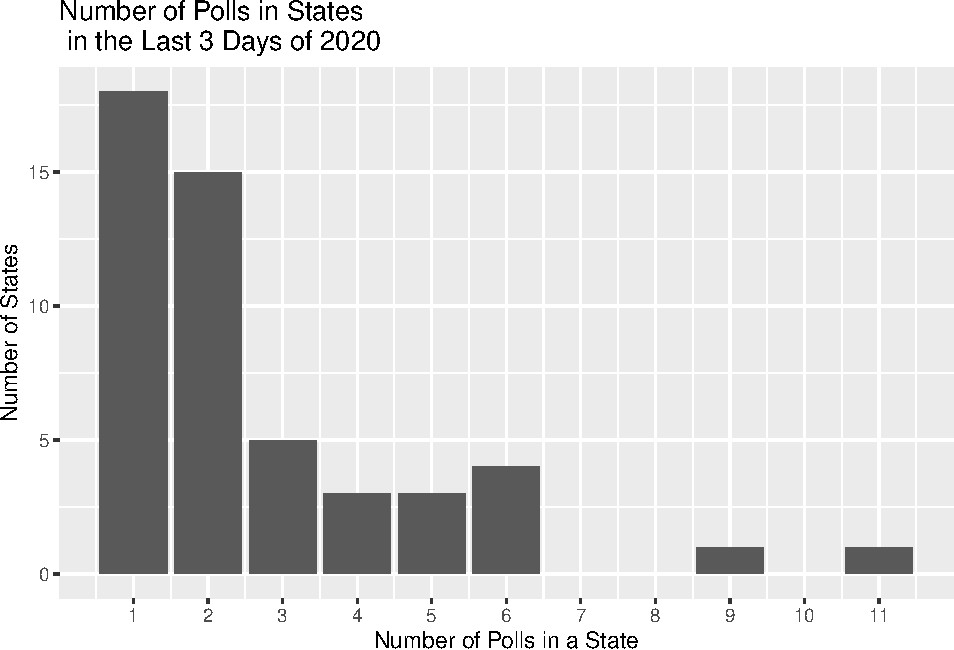
\includegraphics{psc4175_hw_8_files/figure-latex/unnamed-chunk-32-1.pdf}

\end{document}
